\documentclass[a4paper,14pt]{extarticle}
\usepackage[T2A]{fontenc}
\usepackage[utf8]{inputenc}
\usepackage[english,russian]{babel}

\usepackage[newfloat]{minted}
\usepackage[dvipsnames]{xcolor}
\definecolor{aliceblue}{rgb}{0.94, 0.97, 1.0}
\usepackage{tikz-uml}
\usepackage[normalem]{ulem}
\usepackage{csquotes}


\usepackage[right=15mm, left=25mm, top=15mm, bottom=20mm, nohead]{geometry}

\usepackage{amsmath}
\usepackage{amsthm}
\usepackage{enumitem}
\usepackage{mathtools}
\usepackage{cmap}
\usepackage{array}

\renewcommand{\baselinestretch}{1.2}
\newtheorem*{definition}{Опр}

\DeclareMathOperator*{\VarInstr}{VarInstr}
\DeclareMathOperator*{\offset}{offset}

\usepackage{caption}
%\newenvironment{code}{\captionsetup{type=listing}}{}
\SetupFloatingEnvironment{listing}{name=Листинг}
\newenvironment{longlisting}{\captionsetup{type=listing}}{}

\usepackage{hyperref}
\usepackage{indentfirst}

\usepackage[
	backend=biber, %подключение пакета biber (тоже нужен)
	bibstyle=gost-numeric, %подключение одного из четырех главных стилей biblatex-gost 
	citestyle=numeric-comp, %подключение стиля стиля (а вот!) 
	language=auto, %указание сортировки языков
	babel=other, %указание языков
	sorting=ntvy, %тип сортировки в библиографии
	doi=false, 
	eprint=false, 
	isbn=false, 
	dashed=false, 
	url=false 
]{biblatex}
\addbibresource{library.bib}
\usepackage{bibentry}

\graphicspath{{img/}}

%\DeclareFieldFormat{postnote}{#1} %убирает с. и p. 
%\renewcommand*{\multicitedelim}{\addsemicolon\space} % добавляет точку с запятой и пробел (; ) в перечислении
%\renewcommand*{\postnotedelim}{\addcolon\space}


\title{Эффективная генерация кода для платформы ARM32}
\author{}
\date{}

\begin{document}
	\begin{titlepage}
	\begin{center}	
		\footnotesize
		МИНИСТЕРСТВО ОБРАЗОВАНИЯ И НАУКИ РОССИЙСКОЙ ФЕДЕРАЦИИ 
		
		ФЕДЕРАЛЬНОЕ ГОСУДАРСТВЕННОЕ АВТОНОМНОЕ ОБРАЗОВАТЕЛЬНОЕ УЧРЕЖДЕНИЕ
		ВЫСШЕГО ОБРАЗОВАНИЯ
		
		«НОВОСИБИРСКИЙ НАЦИОНАЛЬНЫЙ ИССЛЕДОВАТЕЛЬСКИЙ ГОСУДАРСТВЕННЫЙ УНИВЕРСИТЕТ»
		
		(НОВОСИБИРСКИЙ ГОСУДАРСТВЕННЫЙ УНИВЕРСИТЕТ, НГУ)
		\vspace{0.25cm}
	\end{center}	
	\normalsize
	
	\noindent
	\begin{tabular}{l @{\hskip 1cm} l}
		Факультет &Информационных технологий \\
		Кафедра   &Систем информатики 
	\end{tabular}
	
	\vspace{0.5cm}
	
	\noindent
	\hskip 0.2cm Направление подготовки \hskip 0.3cm 09.03.01 Компьютерные науки и системотехника
	
	\vfill		
	
	\begin{center}
		\small	
		\textbf{ВЫПУСКНАЯ КВАЛИФИКАЦИОННАЯ РАБОТА БАКАЛАВРА}\\[4mm]
		\normalsize
		\uline{\hfill  Мерзляков Илья Алексеевич \hfill} 
		
		
		\normalsize
		Тема работы: 
		Разработка бэкенда LLVM для процессора CDM16
		%\bigskip		
	\end{center}
	\vfill
	
	\noindent
	\begin{tabular*}{\textwidth}{l @{\hskip 4cm} l}
		\textbf{\textquote{К защите допущена}}	& \textbf{Научный руководитель} \\
		& \\
		Заведующий кафедрой,		& Доцент ФФ НГУ \\ 
		д.ф.-м.н., профессор		&  \\ 
		& \\
		\uline{Лаврентьев М.М.}/\uline{\hspace{2cm}} & \uline{Иртегов Д.В.}/\uline{\hspace{2cm}} \\ [-1.1ex]
		\scriptsize (фамилия, И.,О.) \hspace{0.5cm} (подпись, МП) & \scriptsize (фамилия, И.,О.) \hspace{0.5cm} (подпись, МП) \\
		& \\ 
		«...»...............20...г.& «...»...............20...г. 			
		
	\end{tabular*}
	\vfill
	\hfill
	\begin{minipage}{0.5\textwidth}
		Дата защиты: «...».............20...г.
	\end{minipage}
	
	\vfill
	
	\begin{center}
		Новосибирск, 2024 г.
	\end{center}
\end{titlepage}
	
	

\tableofcontents

\pagebreak

\section{Введение}

На ФИТ НГУ на курсе «Цифровые платформы» студентами изучается учебный 8-битный процессор CdM8. Из-за ограничений его архитектуры (8-битное адресное пространство, позволяющее использовать только 256 байт памяти), CdM8 не подходит для реализации на нем сложных проектов. В 2023 году группой студентов 3 курса ФИТ НГУ на основе этого процессора был разработан 16-битный процессор CdM16, имеющий 16-битное адресное пространство и позволяющий реализовывать более сложные проекты. Однако, написание кода на языке ассемблера – трудоемкая задача, значительно увеличивающая время разработки, а реализаций высокоуровневых языков для CdM16 в настоящий момент не существует.

В связи с этим было решено создать компилятор языка Си для процессора CdM16.

\pagebreak
\section{Обзор вариантов создания компилятора Си под новую архитектуру}

Есть два способа получить компилятор Си под новую архитектуру: разработать этот компилятор с нуля, или добавить поддержку новой архитектуры в уже существующий компилятор. Для выбора оптимального подхода сначала рассмотрим стадии компиляции программ на Си.

% SRC: https://habr.com/ru/articles/478124/
Процесс компиляции программ на языке Си состоит из нескольких этапов:
\begin{itemize}
	\item Препроцессинг - обработка директив препроцессора (начинаются с '\#')
	\item Компиляция - преобразование отдельных единиц трансляции в ассемблер целевой платформы
	\item Ассемблирование - преобразование ассемблера в машинный код
	\item Компоновка - связывание результатов компиляции отдельных единиц трансляции в единый исполняемый файл
\end{itemize}

Последние два этапа уже реализованы авторами CdM16 в инструменте cocas, поэтому новому компилятору будет достаточно выполнять только препроцессинг и компиляцию. 

\subsection{Свой компилятор}

Компиляция программы на языке Си тоже состоит из нескольких этапов, и не все они зависят от целевой платформы:
препроцессинг, парсинг исходного кода, проверка типов и проведение некоторых оптимизаций производятся одинаково 
для всех архитектур, поэтому создание компилятора "с нуля" будет тратой ресурсов. 
Поэтому оптимальнее будет взять существующий компилятор, поддерживающий несколько архитектур, и добавить в него
поддержку CdM16.

\subsection{PPCI}

\href{https://github.com/windelbouwman/ppci}{PPCI (Pure Python Compiler Infrastructure)} - компилятор языка Си под различные архитектуры. Попытка добавить в него поддержку CdM16 ранее предпринималась создателем CdM16 Николаем Репиным. Из-за низкого качества кода PPCI и отсутствия поддержки (проект не обновляется уже 3 года) попытка завершилась неудачей.

\subsection{GCC}

TODO: Он старый, страшный, написан на Си.

\subsection{LLVM/CLANG}

TODO: Это круто, очень круто

\pagebreak
\section{Обзор архитектуры LLVM}

Изначально проект LLVM создавался как фреймворк для компиляции и \emph{оптимизации программ во время исполнения} с помощью анализа во время выполнения и JIT-компиляции\cite{LLVM:CGO04}. В настоящее время LLVM используется и развивается как инфраструктура для AOT компиляции.
% https://www.researchgate.net/figure/LLVM-Compiler-Development-architecture_fig2_334167635
\begin{figure}[!h]
	\begin{center}
		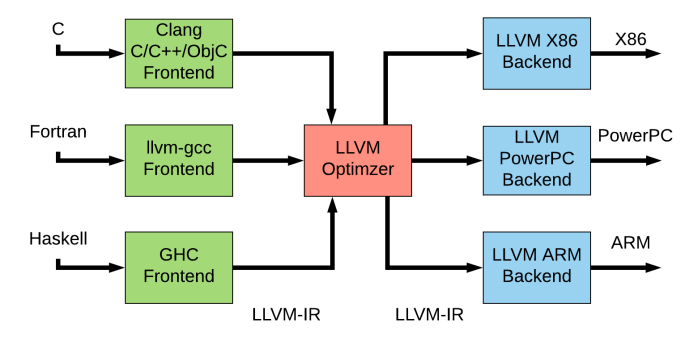
\includegraphics[width=\textwidth]{LLVM-Compiler-Development-architecture.png}
		\caption{Архитектура LLVM \cite{llvmpic}}
	\end{center}
\end{figure}

LLVM состоит из 3-х частей: фронтенда, транслирующего код на языке программирования в \emph{промежуточное представление} (IR), оптимизатора, производящего машинно-независимые оптимизации над IR, и бэкенда, транслирующего IR в инструкции целевой платформы. Так как фронтенд и оптимизатор не зависят от архитектуры, нам % кому нам я здесь одлин
понадобится разработать только бэкенд.

TODO: написать про IR % TODO: IR
TODO: написать про tablegen

\subsection{Архитектура бэкенда LLVM}
% https://llvm.org/docs/CodeGenerator.html#the-targetlowering-class
% https://llvm.org/docs/WritingAnLLVMBackend.html#instruction-relation-mapping

% TODO: операция - не самое подходящее слово
Бэкенд работает с IR в форме DAG (Direct Acyclic Graph) - графа, вершинами которого являются данные и операции над ними, а рёбрами - зависимость одних операций от результатов других. В основном вершины графа соответствуют операциям из IR, однако не весь IR автоматически представим в виде DAG. Некоторые операции, такие как вызов функций, получение их результата, получение значений параметров функции бэкенд должен 'спустить' (lower) в граф. Также не все операции и типы данных IR могут поддерживаться архитектурой (например, CdM16 не поддерживает 8-битные числа в регистрах), бэкенд должен 'легализовать' такие операции, т.е. заменить их несколькими поддерживаемыми операциями. % TODO: плохое предложение

После построения DAG происходит \emph{выбор} (selection) инструкций, этим занимается \emph{SelectionDAG}. Инструкции целевой платформы описываются на специальном языке \emph{tablegen}. Tablegen позволяет компактно задать мнемонику инструкции, её входные и выходные регистры и шаблон (pattern) из вершин DAG, которому она соответствует. Большинство инструкций автоматически выбираются на основе шаблонов, однако некоторые нужно выбирать вручную.

% TODO: как-то плоховато
После выбора инструкций бэкенд должен вывести их в текстовый ассемблерный файл. Части LLVM, ответственные за это, заточены под синтаксис GAS, который значительно отличается от ассемблера CdM16 \emph{cocas}, поэтому нам необходимо изменить логику вывода ассемблерного кода.


\pagebreak
\section{Обзор архитектуры CdM16}

% SRC: https://github.com/cdm-processors/cdm-devkit/blob/master/docs/cdm16/cdm16-overview.md
CdM16 - это 16-битный Load-Store процессор, разработанный студентами НГУ для использования на курсе "Цифровые платформы". Основные технические характеристики:
\begin{itemize}
	\item 8 16-битных регистров общего назначения
	\item возможность адресовать 64 кБ адресного пространства
	\item арифметические инструкции принимают 3 операнда - 2 регистра-источника и регистр назначения
\end{itemize}

\pagebreak
\section{Реализация бэкенда LLVM для CdM16}
\subsection{Описание архитектуры}
В первую очередь необходимо описать основные характеристики архитектуры: размеры типов данных и набор регистров. Первое описывается с помощью строки DataLayout. Для CdM16 эта строка выглядит так: \mint{text}|e-S16-p:16:16-i8:8-i16:16-m:C-n16| % TODO: ссылка на доку https://llvm.org/docs/LangRef.html#data-layout
Данный набор символов означает, что:
\begin{itemize}
	\item платформа little-endian
	\item стэк выровнен по 2 байта
	\item размер указателя - 2 байта
	\item переменные в памяти выравнивать не нужно
	\item платформа поддерживает арифметические операции только с 16-битными числами
\end{itemize}

Набор регистров описан на языке tablegen в файле CDMRegisterInfo.td. У CdM16 8 регистров общего назначения, которые объединены в класс CPURegs:
\begin{minted}[breaklines]{text}
def CPURegs : RegisterClass<"CDM", [i16], 8, (add R0, R1, R2, R3, R4, R5, R6, FP)>;
\end{minted}
Объявление класса регистров необходимо для работы аллокатора регистров LLVM

\subsection{Описание инструкций}
Все инструкции CdM16 также описаны на tablegen и наследуются от класса CDMInst:
\mint[breaklines]{text}|class CDMInst<dag outs, dag ins, string asmstr, list<dag> pattern>: Instruction|

Параметры outs и ins определяют, какие регистры использует и изменяет инструкция; параметр instr\_asm задаёт мнемонику инструкции, параметр pattern задаёт шаблоны в SelectionDAG, которым соответствует инструкция. Большая часть инструкций наследуются от CDMInst не напрямую, а через другие классы.

Большинство арифметических инструкций наследуются от класса arithLogicR:
\begin{minted}[breaklines]{text}
class arithLogicR<string asm_instr, SDNode OpNode>:
  CDMInst<(outs CPURegs:$rd), (ins CPURegs:$rs0, CPURegs:$rs1),
    !strconcat(asm_instr, " $rs0, $rs1, $rd"),
    [(set CPURegs:$rd, (OpNode CPURegs:$rs0, CPURegs:$rs1))]>{
		// Некоторые параметры пропущены для краткости
}

def ADD: arithLogicR<"add", add>;
def SUB: arithLogicR<"sub", sub>;
// Также AND, OR, XOR
\end{minted}

Класс arithLogicR описывает инструкцию, имеющую два входных операнд-регистра и один выходной, и попадающую под шаблон "сохранить в регистр результат выполнения операции-параметра над входными регистрами". Инструкции, использующие этот класс, просто задают операцию для шаблону и мнемонику.

CdM16 также поддерживает инструкции сложения и вычитания с константой, они реализованы через класс arithLogicRi, в котором одним из параметров вместо регистра является immediate-значение (константа).

Битовые сдвиги в CdM16 не соответствуют битовым сдвигам в LLVM. Во-первых, в CdM16 нет инструкции сдвига на переменное кол-во бит, т.е. код \mintinline{c}|i << j| не скомпилируется. Эту проблему достаточно легко решить с помощью таблицы поиска, это будет сделано в новых версиях бэкенда. Также CdM16 может сдвигать не более, чем на восемь бит за раз. Эта проблема решается созданием мультикласса, добавляющего, в зависимости от константного аргумента, нужно ли добавлять дополнительную инструкцию сдвига:
\begin{minted}[breaklines]{text}
def imm1_8: ImmLeaf<i16, [{return (Imm >= 1) && (Imm <= 8);}]>;
def imm9_16: ImmLeaf<i16, [{return (Imm >= 9) && (Imm <= 16);}]>;
multiclass ShiftImm<string instr_asm, SDNode OpNode> {
 let Defs = [PSR] in {
	def _1_8 : CDMInst<(outs CPURegs:$rd), (ins CPURegs:$rs, shamt:$shamt),
	!strconcat(instr_asm, "\t$rs, $rd, $shamt"),
	[(set CPURegs:$rd, (OpNode CPURegs:$rs, imm1_8:$shamt))]>;
	
	def _9_16 : CDMInst<(outs CPURegs:$rd), (ins CPURegs:$rs, shamt:$shamt),
	!strconcat(
	!strconcat(instr_asm, "\t$rs, $rd, 8\n\t"),
	!strconcat(instr_asm, "\t$rd, $rd, $shamt-8")
	),
	[(set CPURegs:$rd, (OpNode CPURegs:$rs, imm9_16:$shamt))]>;
  }
}
defm SHL  : ShiftImm<"shl", shl>;
// And so on
\end{minted}

\subsection{Работа с памятью}
CdM16 имеет 3 основных способа адресации памяти:
\begin{itemize}
	\item адрес в регистре
	\item адрес равен сумме двух регистров (полезно при доступе к элементам массивов и полям структур)
	\item адрес равен сумме значения регистра FP и константы (полезно для доступа к переменным на стеке)
\end{itemize}

Выбор между режимами адресации реализован не через tablegen, а в файле CDMIselDAGToDAG.cpp. Инструкции для разнух способов адресации имеют разные паттерны адреса, LLVM выберет первую инструкцию, паттерн которой совпал с частью SelectionDAG. Второй режим выбирается, если % TODO: мб картинку сюда
адрес является суммой двух значений, иначе выбирается первый режим. Третий режим используется только для доступа к стеку.

\subsection{Стэк и соглашение о вызовах}
CdM16 поддерживает адресацию относительно регистра FP (frame pointer, он же r7), поэтому для бэкенда он считается зарезервированным, в нем всегда хранится указатель на начало стекового кадра.
\begin{table}[!h]
	\begin{center}
		\begin{tabular}{ |c|c| }
			\hline
			Адрес & Содержимое \\
			\hline
			 & Предыдущий кадр \\
			 FP+2 & Адрес возврата \\
			 FP & Сохранённый FP \\
			 FP-2 .. SP & Локальные переменные \\
			 \hline
		\end{tabular}
		\caption{Структура стекового кадра (стек растёт вниз)}
	\end{center}
\end{table}

Каждая функция, использующая стек, имеет пролог и эпилог, создающие стековый кадр и восстанавливающие предыдущий:
\begin{minted}{asm}
# Пролог
pusр  fp # сохранить старое значение fp
ldsp  fp # загрузить в fp указатель на вершину стека
addsp N  # выделить на стеке N байт под локальные переменные
# Эпилог
addsp  N   # вернуть вершину стека обратно
pop    fp  # восстнанвить старое значение fp
\end{minted}
% TODO: ограничения lsw/ssw

Соглашение о вызовах в данный момент позволяет передать до 4-х числовых параметров (в т.ч. указателей) в регистрах r0-r3, и возвращать одно числовое значение. Передача структур по значению и дополнительных числовых аргументов не поддерживается, но запланирована, она будет реализована записью на стек вызывающей функцией.

\subsection{Вызов функций}

Поддержка вызова функций должна быть реализована в двух местах: при генерации кода вызывающей функции, и при генерации пролога и эпилога вызываемой функции.

Генерация кода вызова функции реализована в файле CDMISelLowering.cpp. Метод LowerCall генерирует код, размещающий аргументы в регистрах r0-r3, и на основании соглашения о вызовах определяет список регистров, которые должна сохранить вызывающая функция. Затем метод LowerCallResult вносит результат вызова в SelectionDAG функции (для текущего соглашения о вызовах это заключается в копировании данных из регистра r0).

Генерация обработки аргументов вызываемой функции также реализована в CDMISelLowering.cpp. Метод LowerFormalArguments вносит аргументы в SelectionDAG с помощью DAG.getCopyFromReg. Метод LowerReturn с помощью DAG.getCopyToReg помещает возвращаемое значение в регистр r0.

Методы SelectionDAG getCopyFromReg и getCopyToReg не всегда генерируют код, копирующий значения, они сообщают LLVM, что значение находится в определённом регистре или оно должно оказаться в определённом регистре.


\subsection{Инструкции условного перехода}

Условия оператора if и циклов компилируются в вершину BR\_CC SelectionDAG. У этой вершины аргументами являются condition code (код условия), два значения для сравнения и базовый блок, в который нужно перейти, если условие выполнено. Обработка условных переходов реализована в методе CDMDagToDagIsel::SelectConditionalBranch.
\begin{table}[!h]
	\begin{center}
		\begin{tabular}{ |l|l|l|  }
			\hline
			LLVM & CdM16 & Значение \\
			\hline
			SETLT & blt & < \\
			SETLE & ble & <= \\
			SETGT & bgt & > \\
			SETGE & bge & >= \\
			SETULT & blo & беззнаковое < \\
			SETULE & bls & беззнаковое <= \\
			SETUGT & bhi & беззнаковое > \\
			SETUGE & bhs & беззнаковое >= \\
			SETEQ & beq & ==\\
			SETNE & bne & != \\

			\hline
		\end{tabular}
		\caption{Соответствие кодов условия LLVM инструкциям условного перехода CdM16}
	\end{center}
\end{table}
Условный переход всегда раскрывается в последовательность инструкций cmp и b*. У такого подхода есть недостаток: из-за особенностей аллокатора регистров LLVM между любыми двумя инструкциями может быть вставлена инструкция move. Так как на CdM16 эта инструкция меняет флаги состояния процессора, устанавливаемые cmp, вставка её между cmp и b* некорректна. В данный момент в качестве временного решения вместо инструкции move используется макрос movens, раскрывающийся в последовательность push, pop. В будущем для решения этой проблемы планируется % TODO ссылка на коммент в гугл группах из чата с Николаем
объединить инструкции cmp и b* в одну, чтобы LLVM не мог вставлять инструкции между ними.

\subsection{Оператор switch}

Оператор switch компилируется либо в несколько условных переходов, либо в таблицу поиска. Это делает clang/llvm. Для работы таблиц поиска потребовалось найти и исправить в коде LLVM место, где генерируются названия этих таблиц, так как ассемблер cocas не поддерживает (на момент написания) точку в названиях символов.

\subsection{Тернарный оператор}

Тернарный оператор и некоторые другие конструкции раскрываются LLVMом в вершины трех типов:
\begin{itemize}
	\item select - выбрать одно из двух значений на основании boolean аргумента
	\item setcc - проверить условие на двух аргументах и вернуть boolean значение
	\item select\_cc - setcc + select - проверить условие и выбрать одно из двух значений
\end{itemize}

Так как в CdM16 отсутствуют conditional move инструкции, в которые удобно раскрывать select, и инструкции, в которые удобно раскрывать setcc, в бэкенде реализована обработка только select\_cc, а LLVM настроен автоматически раскрывать select и setcc в select\_cc. % TODO: список терминов в описании архитектуры LLVM

В методе CDMISelLowering::EmitInstrWithCustomInserter реализовано раскрытие select\_cc. Так как select\_cc раскрывается в уловный переход, выбрать его с помощью tablegen нельзя. Для раскрытия необходимо разделить базовый блок на две части, и добавить еще один. Переход из первой половины (HeadBB) во вторую (TailBB) напрямую происходит, если условие истинно, иначе происходит переход в дополнительный базовый блок (FalseBB), за которым следует TailBB. В HeadBB добавляется только инструкция сравнения и прыжка, в FalseBB ничего не добавляется, а в TailBB добавляется % TODO: сюда бы ссылку на описание фи-ноды
$\phi$-нода. Инструкции move и безусловные переходы LLVM вставляет автоматически.

\begin{figure}[h!] % TODO: minted inside tikz, better arrows, better positioning
	\begin{center}
		\begin{tikzpicture}[
			squarednode/.style={rectangle, draw=black, very thick, minimum size=5mm,align=left},
			]
			\node[squarednode] (headbbnode) at (0, 0) {\textbf{HeadBB} \\ cmp r*, r* \\ b* TailBB };
			\node[squarednode] (falsebbnode) at (5, -3) {\textbf{FalseBB}};
			\node[squarednode] (tailbbnode) at (0, -6) {\textbf{TailBB} \\ phi(rTrue, HeadBB, rFalse, FalseBB)};
			
			\draw[->] (headbbnode.south) -- (falsebbnode.north);
			\draw[->] (headbbnode.south) -- (tailbbnode.north);
			\draw[->] (falsebbnode.south) -- (tailbbnode.north);
		\end{tikzpicture}
		\caption{Результат раскрытия select\_cc}
	\end{center}
\end{figure}

В результате код вида \mintinline{c}|int f(int a){return a > 15 ? 1337 : 228;}| компилируется в
\begin{minted}{asm}
f>
# %bb.0: (HeadBB)
movens	r0, r1
ldi	r0, 1337
ldi	r2, 15
cmp	r1, r2
bgt	__LBB0_2
# %bb.1: (FalseBB)
ldi	r0, 228
__LBB0_2: # (TailBB)
rts
\end{minted}


\subsection{Линковка}
\subsection{Обработчики прерываний}

\pagebreak
\section{Заключение}

В результате работы был создан компилятор языка Си для платформы CdM16, поддерживающий значительное подмножество возможностей языка Си: создание функций, принимающий до 4 числовых аргументов, 8- и 16-битные переменные, циклы, ветвления, структуры, массивы, глобальные переменные, статические и внешние символы.

Пример проекта, написанного на Си под CdM16 - \href{https://github.com/leadpogrommer/llvm-project-cdm/tree/backend/cdm/llvm/test_cdm/life_multifile}{реализация игры "жизнь"}.

\subsection{Планы на будущее}

В будущем планируется реализовать:
\begin{itemize}
	\item программную реализацию 32-битной арифметики
	\item поддержку передачи аргументов на стеке
	\item поддержку функций с переменным количеством аргументов (vararg)
	\item минимальную стандартную библиотеку Си
\end{itemize}


\pagebreak
\printbibliography
\addcontentsline{toc}{section}{\refname}




	
\end{document}